\documentclass[useAMS,usenatbib]{mn2e}
\usepackage{footnote}
\usepackage{graphicx}
\usepackage{amsmath}
\usepackage{natbib}
\usepackage{array}
\usepackage{color}
\usepackage{url}
\voffset=-0.5in

\definecolor{nc}{rgb}{0,0,0}
\def\changed    {\color{nc} }

\def\starpy {\textsc{starpy}}

\begin{document}
\title[Quenching by AGN]{Galaxy Zoo: Evidence for quenching caused by AGN feedback}
\author[Smethurst et al. 2014]{R. ~J. ~Smethurst,$^{1}$ C. ~J. ~Lintott,$^{1}$ B. ~D. ~Simmons,$^{1}$
\\ $^1$ Oxford Astrophysics, Department of Physics, University of Oxford, Denys Wilkinson Building, Keble Road, Oxford, OX1 3RH, UK 
\\
}

\maketitle

\begin{abstract}
Evidence of recent quenching in galaxies with AGN. New Bayesian SFH tool \starpy let's us investigate the SFH as two parameters $[t, \tau]$ and investigate the parameter likelihood in this space of active and inactive galactic nuclei. We find that galaxies currently hosting an AGN have undergone very recent rapid quenching across all mass bins. This is not seen in those galaxies without current AGN.  \footnotemark[1]

\end{abstract}

\footnotetext[1]{This investigation has been made possible by the participation of more than 250,000 users in the Galaxy Zoo project. Their contributions are individually acknowledged at \url{http://authors.galaxyzoo.org}}

\section{Introduction}

There is clearly a relationship between central black hole and evolution of galaxy. Magorrian relation shows this as do simulations and observations of feedback. 

This effect seems to be strongest during AGN phase of black hole growth. 

Theorised that AGN can have negative feedback on galaxy SFR. This is supported by the observational evidence that the largest fraction of AGN are found in green valley, suggesting some link to the process of quenching star formation in order for a galaxy to progress from the blue cloud to the red sequence. 

Here we find indirect observational evidence linking the star formation history (SFH) of a galaxy to the presence of a current AGN with the use of a novel new code implementing a Bayesian method; \starpy. Given NUV and optical colours and using SSP models, \starpy can effectively describe the SFH of a galaxy with two parameters. 

Through this approach, we aim to determine the following:
\begin{enumerate}
\item{Are galaxies currently hosting an AGN undergoing quenching?}
\end{enumerate}

This paper proceeds as follows. Section 2 contains a description of the sample data, which is used in the Bayesian analysis of an exponentially declining star formation history model. Section 3 contains the results produced by this analysis, with Section 4 providing a detailed discussion of the results obtained. We also summarise our findings in Section 6. The zero points of all ugriz magnitudes are in the AB system and where necessary we adopt the WMAP Seven-Year Cosmological parameters (Jarosik et al. 2011) with (�m , �? , h) = (0.26, 0.73, 0.71).


\section{Data}

\subsection{Galaxy Zoo 2}\label{galzoo}

\begin{figure*}
\centering{
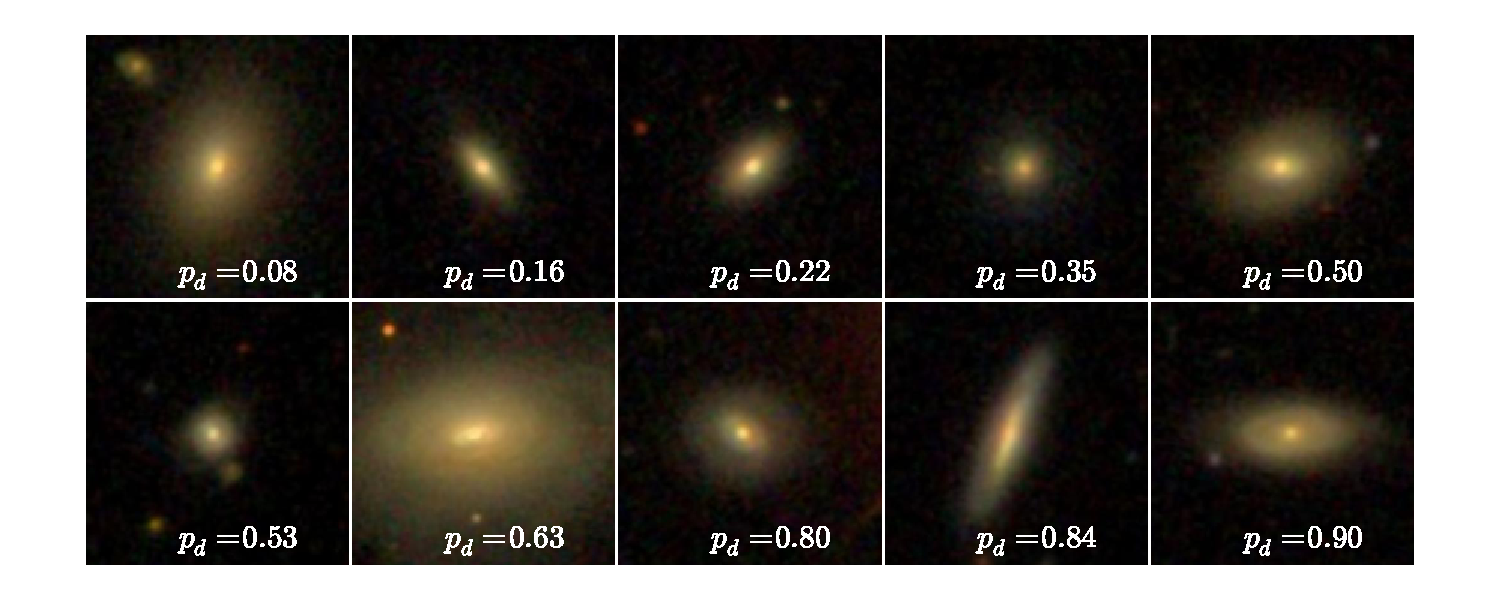
\includegraphics[width=\textwidth]{mosaic_agn_seyfert_disc_fraction.pdf}}
\caption{Randomly selected SDSS \emph{gri} composite images from the sample of $439$ narrow-line AGN showing the continuous probabilistic nature of the Galaxy Zoo sample from a redshift range $0.040 < z < 0.045$. The debiased `disc or featured' vote fraction (see \citealt{GZ2}) for each galaxy is shown. The scale for each image is $0.099~\rm{arcsec/pixel}$.}
\label{mosaic}
\end{figure*}

In this investigation we use visual classifications of galaxy morphologies from the Galaxy Zoo 2\footnote{\url{http://zoo2.galaxyzoo.org/}} citizen science project \citep{GZ2}, which obtains multiple independent classifications for each optical galaxy image; the full question tree for each image is shown in Figure 1 of \citealt{GZ2}.  

The Galaxy Zoo 2 (GZ2) project consists of $304, 022$ images from the SDSS DR8 (a subset of those classified in Galaxy Zoo 1; GZ1) all classified by \emph{at least} 17 independent users, with the mean number of classifications standing at $\sim42$.

Further to this, we required NUV photometry from the GALEX survey, within which $\sim42\%$ of the GZ2 sample were observed, giving a total sample size of $126, 316$ galaxies. The completeness of this subsample of GZ2 matched to GALEX is shown in Figure 2 of \cite{Sme2015} with the $u$-band absolute magnitude against redshift for this sample compared with the SDSS data set. Typical Milky Way $L_*$ galaxies with $M_u \sim -20.5$ are still included in the GZ2 subsample out to the highest redshift of $z \sim 0.25$; however dwarf and lower mass galaxies are only detected at the lowest redshifts.


\subsection{\sc{STARPY}}

\starpy~ is a \textsc{python} code which allows the user to derive the quenched star formation history (SFH) of a galaxy through a Bayesian Markov Chain Monte Carlo method through the input of two observed photometric colours and a redshift, and the use of the SSP models of \citep{BC03}. The star formation history template is an exponential decline of the SFR and is described by two parameters $[t_q, \tau]$ where $t$ is the time at which the onset of quenching begins $[Gyr]$ and $\tau$ is the exponential rate at which quenching occurs $[Gyr]$. Under the simplifying assumption that all galaxies formed at $t=0$ Gyr with an initial burst of star formation, the SFH can therefore be described as: 

\begin{equation}\label{sfh}
SFR =
\begin{cases}
i_{sfr}(t_q) & \text{if } t < t_q \\
i_{sfr}(t_q) \times exp{\left( \frac{-(t-t_{q})}{\tau}\right)} & \text{if } t > t_q 
\end{cases}
\end{equation}

where $i_{sfr}$ is an initial constant star formation rate dependent on $t_q$.  A smaller $\tau$ value corresponds to a rapid quench, whereas a larger $\tau$ value corresponds to a slower quench. The output of \starpy is probabilistic in nature and provides the likelihood across the entirety of the two parameter space for each individual galaxy. These individual galaxy likelihoods can be combined to visualise the areas of high probability in the model parameter space for a given population of galaxies (e.g. the green valley as in \citealt{Sme2015} and here with active and inactive galaxies). The GZ2 data also provides uniquely powerful continuous measurements of a galaxy�s morphology, therefore we utilise the user vote fractions to obtain separate model likelihood parameter distributions for both smooth and disc galaxies; obtained by weighting by the morphology vote fraction of each galaxy when combined. We stress that this portion of the methodology is a non-Bayesian visualisation of the combined individual galaxy results for each population.

The probabilistic fitting methods to this SFH for an observed galaxy are described in full detail in \cite{Sme2015} wherein the \starpy ~code was run on a volume limited sample ($0.01 < z < 0.25$)  of $126,316$ galaxies of the Galaxy Zoo 2 project from SDSS DR8 \citep{York2000, Aihara11}. This will be referred to as the {\sc GZ2-starpy} sample. 

\subsection{AGN Sample} 

We utilise a new sample of type 1 AGN selected by \citep{Oh15} who built on the selection techniques of the OSSY catalogue \footnote{http://gem.yonsei.ac.kr/ossy/} described in \citep{Oh11}. To search for broad line region (BLR) AGN \citep{Oh15} used a flux ratio between between two regions near the $H\alpha$ emission line in SDSS DR7 spectra. The two regions were $6460-6480 \AA$ and $6523 - 6543 \AA$ to give a ratio between $F_{6533}/F_{6470}$; which if high identified those candidate galaxies which could currently hosting an AGN. Each spectra was fit using the {\sc IDL ppxf} and {\sc gandalf} programs with the \citep{BC03} and {\sc MILES} stellar libraries using the Levenberg Marquardt minimisation method \citep{Mark09}. From the measured continuums and emission line widths type 1 AGN were selected with the following criteria:

\begin{enumerate}
\item{$0.00 < z < 0.20$}
\item{FWHM of $H\alpha > 800 ~\rm{km~s^{-1}}$}
\item{A/N of broad $H\alpha > 3$}
\end{enumerate}

This resulted in a sample of 9,671 type 1 AGN identified by cite{Oh15} with broad line and luminosity measurements provided in the published catalogue. This sample was then matched to the {\sc GZ2-starpy} sample to give $1,357$ galaxies currently hosting AGN. This sample is studied in three different mass bins with $202$ low mass ($M_* < 10.25 M_{\odot}$), $756$ medium mass  ($ 10.25 < M_* [M_{\odot}] < 10.75 $) and $399$ high mass ($M_* > 10.75 M_{\odot}$) galaxies. 

\section{Results}

Across different mass bins in Figure \ref{agn} compared to Figure {inactive} we see an increase in the likelihoood across the parameter space for rapid quenching at recent times for AGN hosting galaxies. 

\begin{figure*}
\includegraphics[width=0.4\textwidth]{sum_weight_low_mass_smooth_agn_oh_sample.png}
\includegraphics[width=0.4\textwidth]{sum_weight_low_mass_disc_agn_oh_sample.png}
\includegraphics[width=0.4\textwidth]{sum_weight_med_mass_smooth_agn_oh_sample.png}
\includegraphics[width=0.4\textwidth]{sum_weight_med_mass_disc_agn_oh_sample.png}
\includegraphics[width=0.4\textwidth]{sum_weight_high_mass_smooth_agn_oh_sample.png}
\includegraphics[width=0.4\textwidth]{sum_weight_high_mass_disc_agn_oh_sample.png}
\caption{SLB plots for galaxies with AGN. Split into low (top), medium (middle) and high (bottom) mass galaxies which are weighted by their GZ2 vote fraction for either smooth (left) or disc (right) galaxies.}
\label{agn}
\end{figure*}

\begin{figure*}
\includegraphics[width=0.4\textwidth]{oh_sample/sum_weight_low_mass_smooth_no_agn_oh_sample.png}
\includegraphics[width=0.4\textwidth]{oh_sample/sum_weight_low_mass_disc_no_agn_oh_sample.png}
\includegraphics[width=0.4\textwidth]{oh_sample/sum_weight_med_mass_smooth_no_agn_oh_sample.png}
\includegraphics[width=0.4\textwidth]{oh_sample/sum_weight_med_mass_disc_no_agn_oh_sample.png}
\includegraphics[width=0.4\textwidth]{oh_sample/sum_weight_high_mass_smooth_no_agn_oh_sample.png}
\includegraphics[width=0.4\textwidth]{oh_sample/sum_weight_high_mass_disc_no_agn_oh_sample.png}
\caption{SLB plots for galaxies which are inactive. Split into low (top), medium (middle) and high (bottom) mass galaxies which are weighted by their GZ2 vote fraction for either smooth (left) or disc (right) galaxies.}
\label{agn}
\end{figure*}


\section{Discussion}

Rapid quench results in high luminosity AGN?

Slow quench results in low luminosity AGN?

Majority of disc galaxies with AGN found at slow quenching timescales but with low luminosity AGN?

Small fraction of AGN are in smooth galaxies found at rapid quenching timescales with high luminosity AGN?

How significant is the quenching? Is this a sample where AGN feedback was important or just one where it happened.

How many galaxies (as discussed earlier) - are they unusual?

Is this a significant chunk of a galaxy population?

Are there AGN out there somewhere which aren't quenching?

\section{Conclusion}

AGN and SFH linked. Rapid == high luminosity but there's not a lot of those. Slow == low luminosity and there's loads of those. Clear evidence for quenching driven by AGN - negative feedback. 

\section*{Acknowledgements}

RS acknowledges funding from the Science and Technology Facilities Council Grant Code ST/K502236/1. BDS gratefully acknowledges support from the Oxford Martin School, Worcester College and Balliol College, Oxford. KS gratefully acknowledges support from Swiss National Science Foundation Grant PP00P2\_138979/1.

The development of Galaxy Zoo was supported in part by the Alfred P. Sloan Foundation. Galaxy Zoo was supported by The Leverhulme Trust. 

Based on observations made with the NASA Galaxy Evolution Explorer.  GALEX is operated for NASA by the California Institute of Technology under NASA contract NAS5-98034

Funding for the SDSS and SDSS-II has been provided by the Alfred P. Sloan Foundation, the Participating Institutions, the National Science Foundation, the U.S. Department of Energy, the National Aeronautics and Space Administration, the Japanese Monbukagakusho, the Max Planck Society, and the Higher Education Funding Council for England. The SDSS Web Site is \url{http://www.sdss.org/}.
The SDSS is managed by the Astrophysical Research Consortium for the Participating Institutions. The Participating Institutions are the American Museum of Natural History, Astrophysical Institute Potsdam, University of Basel, University of Cambridge, Case Western Reserve University, University of Chicago, Drexel University, Fermilab, the Institute for Advanced Study, the Japan Participation Group, Johns Hopkins University, the Joint Institute for Nuclear Astrophysics, the Kavli Institute for Particle Astrophysics and Cosmology, the Korean Scientist Group, the Chinese Academy of Sciences (LAMOST), Los Alamos National Laboratory, the Max-Planck-Institute for Astronomy (MPIA), the Max-Planck-Institute for Astrophysics (MPA), New Mexico State University, Ohio State University, University of Pittsburgh, University of Portsmouth, Princeton University, the United States Naval Observatory, and the University of Washington.

This publication made extensive use of the Tool for Operations on Catalogues And Tables (TOPCAT; ~\citealt{Taylor05}) which can be found at \url{http://www.star.bris.ac.uk/~mbt/topcat/}. Ages were calculated from the observed redshifts using the \emph{cosmolopy} package provided in the Python module \emph{astroPy}\footnote{\url{http://www.astropy.org/}}; \citealt{Rob13}). This research has also made use of NASA's ADS service and Cornell's ArXiv. 

\begin{thebibliography}{}

\bibitem[\protect\citeauthoryear{Aihara et al.}{2011}]{Aihara11} Aihara, H. et al., 2011, ApJSS, 193, 29

\bibitem[\protect\citeauthoryear{Bruzua \& Charlot}{2003}]{BC03} Bruzual, G. \& Charlot, S., 2003, MNRAS, 344, 1000

\bibitem[\protect\citeauthoryear{Lintott et al.}{2008}]{Lintott09} Lintott, C. J. et al., 2008, MNRAS, 389, 1179

\bibitem[\protect\citeauthoryear{Lintott et al.}{2011}]{Lintott11} Lintott, C. J. et al., 2011, MNRAS, 410, 166

\bibitem[\protect\citeauthoryear{Markwardt et al.}{2009}]{Mark09} Markwardt, C. B. 2009, in Astronomical Society of the Pacific Conference Series, Vol. 411, Astronomical Data Analysis Software and Systems XVIII, ed. D. A. Bohlender, D. Durand \& P. Dowler, 251

\bibitem[\protect\citeauthoryear{Oh et al.}{2011}]{Oh11} Oh, K., Sarzi, M., Schawinski, K., \& Yi, S. K., 2011, ApJS, 195, 13

\bibitem[\protect\citeauthoryear{Oh et al.}{2015}]{Oh15} arXiv: 1504.07247

\bibitem[\protect\citeauthoryear{Robitaille et al.}{2013}]{Rob13} Robitaille, T. P. et al., 2013, A\&A, 558, A33

\bibitem[\protect\citeauthoryear{Sarzi et al.}{2006}]{Sar2006} Sarzi, M. et al., 2006, MNRAS, 366, 1151
ph
\bibitem[\protect\citeauthoryear{Schawinski et al.}{2007}]{Sch07} Schawinski, et al., 2007, MNRAS, 382, 1415

\bibitem[\protect\citeauthoryear{Schawinski et al.}{2010}]{Sch2010} Schawinski, K. et al., 2010, MNRAS, 711, 284

\bibitem[\protect\citeauthoryear{Smethurst et al.}{2015}]{Sme2015} Smethurst, R. J. et al., 2015, MNRAS, 450, 435

\bibitem[\protect\citeauthoryear{Taylor}{2005}]{Taylor05} Taylor, M. B., 2005, ASP Conference Series, 347

\bibitem[\protect\citeauthoryear{Willett et al.}{2013}]{GZ2} Willett, K. et al., 2013, MNRAS, 435, 2835

\bibitem[\protect\citeauthoryear{York et al.}{2009}]{York2000} York, D. G. et al., 2000, AJ, 120, 1579

\end{thebibliography}{}

\appendix

\end{document}
